\documentclass[numbering=fraction,aspectratio=169]{beamer}


% -------------------------------
% Packages
% -------------------------------
\usepackage{fontspec}
  \setmainfont{Latin Modern Roman}
  \newfontfamily\emoji{NotoColorEmoji}[Renderer=HarfBuzz]
\usepackage{polyglossia}
\usepackage{hyperref}
\usepackage{xspace}
\usepackage{graphicx}
\usepackage{amsmath}
\usepackage{linguex}


% -------------------------------
% Theme and Styling
% -------------------------------
\usetheme[progressbar=frametitle]{metropolis}

% Colors
\definecolor{unicampRed}{RGB}{163,35,41}
\definecolor{SPYellow}{RGB}{255,223,25}
\definecolor{SPBlue}{RGB}{0,0,137}

% Title page logo
\titlegraphic{
  \vspace{6.5cm}
  \hspace{8.1cm}
  \includegraphics[height=0.9cm]{img/logos/logos-regua}
}

% Color theme and font adjustments
\setbeamercolor{frametitle}{fg=white, bg=SPBlue}
\setbeamercolor{title separator}{fg=unicampRed}

\setbeamercolor{block title alerted}{fg=black, bg=unicampRed}
\setbeamercolor{block body alerted}{fg=black, bg=unicampRed!30}
\setbeamercolor{alerted text}{fg=unicampRed}
\setbeamerfont{alerted text}{series=\bfseries}

\setbeamercolor{block title example}{fg=black, bg=SPYellow}
\setbeamercolor{block body example}{fg=black, bg=SPYellow!30}
\setbeamercolor{footline}{fg=gray}
\setbeamercolor{progress bar}{fg=SPYellow}

% Footer
\setbeamertemplate{frame footer}{
  \tiny
  CC BY 4.0 %
  \qquad%
  LET406 | %
  \insertshortauthor~(\insertshortinstitute) | %
  02/10/2025
}


% -------------------------------
% Custom commands
% -------------------------------
\newcommand\IEL{\textsc{iel}\xspace}
\newcommand\IMPATech{\textsc{impa}\,Tech\xspace}
\newcommand\NHST{\textsc{nhst}\xspace}
\newcommand\ThumbsUp{{\emoji 👍}\ }
\newcommand\ThumbsDown{{\emoji 👎}\ }
\newcommand\WarningEmoji{{\emoji ⚠️}\ }
\newcommand\WorldEmoji{{\emoji 🌐}\ }
\newcommand{\FigureCaption}[1]{{\scriptsize #1}}


% -------------------------------
% URLs
% -------------------------------
\def \LicencaURL{https://creativecommons.org/licenses/by-sa/4.0/}
\def \DisciplinaURL{https://rberaldo.quarto.pub/replicabilidade-linguistica/}

% -------------------------------
% Title page metadata
% -------------------------------
\title{Os métodos da psicolinguística: limites da inferência estatística e a questão da (ir)replicabilidade}
\author[Rafael Beraldo]{Rafael Luis Beraldo\\
  {\small
    \texttt{<\href{mailto:rberaldo@unicamp.br}{rberaldo@unicamp.br}>} ou
    \texttt{<\href{mailto:rafael.beraldo@impatech.edu.br}{rafael.beraldo@impatech.edu.br}>}
  }\\[1ex]
  \textbf{\textsc{ufmg} | LET406 -- Linguística como ciência e aspectos biológicos da linguagem}}
\institute{\IEL/Unicamp e \IMPATech}
\date{2 de outubro de 2025}


% -------------------------------
% Main document
% -------------------------------
\begin{document}
\frenchspacing


\begin{frame}[plain]{}
  \titlepage
\end{frame}


%%% Bloco 0: sobre estes slides e o autor.

\begin{frame}{Sobre estes slides}
  \begin{itemize}
  \item Estes slides foram apresentados em uma aula da disciplina \textbf{LET406 -- Tópicos em Letras D: Linguística como ciência e aspectos biológicos da linguagem} ministrada no dia 2 de outubro de 2025, na Faculdade de Letras da \textsc{ufmg}.
  \item Os slides estão disponíveis sob a licença \href{\LicencaURL}{Creative Commons Atribuição 4.0}.
  \end{itemize}
\end{frame}

\begin{frame}{Sobre mim}
  \begin{itemize}
  \item Doutorado em Linguística pela Unicamp metodologia e replicação;
  \item Professor no \IMPATech e pós-doc no \IEL/Unicamp sob Lívia Oushiro;
  \item Atualmente, ministrando curso sobre irreplicabilidade e linguística: \url{\DisciplinaURL}
  \end{itemize}
\end{frame}


%%% Bloco 1: A psicolinguística e seus métodos.
% - Definição de experimento.
% - Método fundamental na psicolinguística.
% - A questão da inferência e Fisher.
% - O que a estatística frequentista faz. (slide com figurinhas)

\section{A psicolinguística e seus métodos}

\begin{frame}{Exemplo de Kantowitz et al. (2009)}
  \begin{columns}
    \column{.59\textwidth}
    \begin{itemize}
    \item<1-> Tarefa: \alert{defender uma mesa na biblioteca} usando apenas métodos não verbais.
    \item<2-> “Método” (ou Variável Independente): \alert{espalhar seus livros e pertences pela mesa} e aguardar até que alguém se sente.
    \item<3-> Medida (ou Variável Dependente): \alert{tempo} que leva para alguém se sentar.
    \end{itemize}

    \uncover<4->{Por que isso \alert{não é} um experimento?}
    \column{.39\textwidth}
    \centering
    \includegraphics[width=\textwidth]{img/table}\\
    {\footnotesize Foto por \href{https://www.flickr.com/photos/jasonmcdermott/5265264116}{Jason McDermott no Flikr}}
  \end{columns}
\end{frame}

\begin{frame}{Definição de experimento}
  A tarefa descrita anteriormente não é um experimento porque não satisfaz os requisitos básicos de um experimento:
  \medskip

  \begin{quote}
    \only<1>{An experiment occurs when the environment is systematically manipulated so that the causal effect of this manipulation on some behavior can be observed.}
    \only<2>{An experiment occurs when the environment is \alert{systematically manipulated} so that the causal effect of this manipulation on some behavior can be observed.}

    \raggedleft
    (Kantowitz et al., 2009, p.~52)
  \end{quote}

  \uncover<2>{Não há a manipulação sistemática do ambiente, operacionalizada como \alert{pelo menos dois níveis de uma variável independente}.}
\end{frame}

\begin{frame}{Mais sobre experimentos}
  Sobre os experimentos, Kantowitz et al. (2009) ainda afirmam que eles:

  \begin{itemize}
  \item Permitem o \alert{controle das variáveis};
  \item Permitem o estabelecimento de \alert{relações causais};
  \item São \alert{mais econômicos} que métodos observacionais;
  \item São conduzidos para comparar teorias (\emph{“critical experiments”}, p.~54) ou gerar hipóteses (\emph{“what-if experiments”}, p.~54).
  \end{itemize}
\end{frame}

\begin{frame}{Ronald Fisher e a estatística frequentista}
  \begin{columns}
    \column{0.45\textwidth}
    Fisher é o autor de influentes obras de estatística, que impactaram as ciências experimentais:

    \begin{itemize}
    \item<1-> \emph{Statistical Methods for Research Workers} (1925)
    \item<2-> \emph{The Design of Experiments} (1935)
    \end{itemize}
    %
    \column{0.45\textwidth}
    \centering
    \only<1>{\includegraphics[height=6cm]{img/methods}}
    \only<2>{\includegraphics[height=6cm]{img/design}}
  \end{columns}
\end{frame}

\begin{frame}{O tratamento formal da indução}
  Fisher (1955) defende que o pensamento indutivo pode atingir \alert{o mesmo estatuto formal} que a dedução tem na lógica:
  \medskip

  \begin{quote}
    \footnotesize
    Logicians, in introducing the terms “inductive reasoning” and “inductive inference” evidently imply that they are speaking of processes of the mind falling to some extent outside those of which a full account can be given in terms of the traditional deductive reasoning of formal logic. \pause
    Deductive reasoning in particular supplies no essentially new knowledge, but merely reveals or unfolds the implications of the axiomatic basis adopted. Ideally, perhaps, it should be carried out mechanically. \pause
    \alert{It is the function of inductive reasoning to be used, in conjunction with observational data, to add new elements to our theoretical knowledge.} \pause
    That such a process existed, and was possible to normal minds, has been understood for centuries; \alert{it is only with the recent development of statistical science that an analytic account can now be given, about as satisfying and complete, at least, as that given traditionally of the deductive processes}.

    \raggedleft
    (Fisher, 1955, p.~74, grifo nosso)
  \end{quote}
\end{frame}

\begin{frame}{O funcionamento da estatística frequentista}
  O que faz a \alert{estatística frequentista}? Ela quantifica a probabilidade de uma \alert{distribuição observada} -- os dados obtidos -- \alert{contra uma distribuição teórica, que é dada}.

  \centering
  \includegraphics[height=4cm]{img/nhst}\\
  \FigureCaption{Vejamos a demonstração em \url{https://rpsychologist.com/d3/nhst/}.}
\end{frame}


%%% Bloco 2: Problemas com a estatística.
% - O problema da interpretação dos resultados.
% - Cohen (1994).
% - Viés de publicação.
% - Ioannidis (2005).

\section{Os limites da inferência estatística frequentista}

\begin{frame}{Críticas ao \NHST (Null Hypothesis Statistical Testing)}
  As críticas ao \NHST têm se acumulado desde os anos 1930; trago aqui apenas Cohen (1994):
  \medskip

  \begin{quote}
    What's wrong with NHST? Well, among many other things, \alert{it does not tell us what we want to know}, and we so much want to know what we want to know that, out of desperation, we nevertheless believe that it does! What we want to know is “Given these data, what is the probability that $H_0$ is true?” But as most of us know, what it tells us is \pause \alert{“Given that $H_0$ is true, what is the probability of these (or more extreme) data?”}

    \raggedleft
    (Cohen, 1994, p.~997)
  \end{quote}
\end{frame}

\begin{frame}{O viés de publicação}
  \begin{columns}
    \column{0.7\textwidth}
    Rosenthal (1979): o famoso \alert{“problema do engavetamento”}; há um \alert{viés de publicação} que favorece estudos “positivos”, introduzindo distorções e até mesmo falsos positivos na literatura.
    \medskip

    \begin{quote}
      \footnotesize
      Both behavioral researchers and statisticians have \alert<1->{long suspected that the studies published in the behavioral sciences are a biased sample of the studies that are actually carried out} (Bakan, 1967; McNemar, 1960; Smart, 1964; Sterling, 1959). The extreme view of this problem, the \alert<2->{“file drawer problem,”} is that the \alert<3->{journals are filled with the 5\% of the studies that show Type I errors}, while the file drawers back at the lab are filled with the 95\% of the studies that show nonsignificant (e.g., \(p > .05\)) results.
    \end{quote}
    \column{0.3\textwidth}
    \centering
    \includegraphics[width=\textwidth]{img/drawer}
    {\footnotesize Por \href{https://x.com/mc\_hankins}{@mc\_hankins}}
  \end{columns}
\end{frame}

\begin{frame}{A maior parte da pesquisa publicada é falsa}
  Ioannidis (2005) publica o seu (agora) influente artigo \emph{Why Most Published Research Findings Are False}.
  \medskip

  \centering
  \includegraphics[height=4cm]{img/ioannidis2005}
\end{frame}

\begin{frame}{O argumento de Ioannidis (2005) ilustrado}

  \centering
  \only<1>{\includegraphics[height=3.5cm]{img/ioannidis2005-ilustrado-cut}}
  \only<2>{\includegraphics[height=3.5cm]{img/ioannidis2005-ilustrado}}\\
  {\footnotesize Ilustração baseada em interpretação de Pashler e Harris (2012). O modelo de Ioannidis (2005) adiciona outras considerações, tais como o baixo poder estatístico, os vieses dos pesquisadores e os múltiplos testes por laboratórios/grupos de pesquisa diferentes. (Fonte: Beraldo, 2024)}
\end{frame}


%%% Bloco 3: A replicação.
% - Papel das replicações (Popper)
% - Definição de replicação (Nosek e Errington, 2020)
% - Importância das replicações (Vasishth e Nicenboim, 2016)

\section{O conceito de replicação}

\begin{frame}{A “reprodução” e a falseabilidade}
  O papel da “reprodução” de uma observação para Popper:
  \medskip

  \begin{quote}
    We must clearly distinguish between \alert<1->{falsifiability and falsification}. […]

    We say that a theory is falsified only if we have accepted basic statements which contradict it […] This condition is necessary, but not sufficient; for we have seen that \alert<2->{non-reproducible single occurrences are of no significance to science}. Thus a few stray basic statements contradicting a theory will hardly induce us to reject it as falsified. \alert<3>{We shall take it as falsified only if we discover a reproducible effect which refutes the theory}.

    \raggedleft
    (Popper, 2002 [1959], p.~66)
  \end{quote}
\end{frame}

\begin{frame}{Uma definição de “replicação”}
  Nosek e Errington (2020) propõem que \alert<1>{a replicação seja fruto de um “acordo”}. \pause Em outras palavras, \alert{quais são as condições necessárias para que uma replicação seja informativa?} \pause
  \bigskip

  \begin{quote}
    \begin{description}
    \item[Definição de replicação] Uma replicação é um estudo cujos resultados, quaisquer que sejam, seriam considerados como evidência para diagnosticar uma alegação de uma pesquisa anterior.
    \end{description}

    \medskip
    \raggedleft
    (Nosek e Errington, 2020, p.~2, tradução nossa)
  \end{quote}
\end{frame}

\begin{frame}{Critérios para uma replicação}
  Nosek e Errington (2020) definem \alert{dois critérios simétricos} para classificar replicações:
  \medskip

  \begin{quote}
    \begin{enumerate}
    \item Resultados \alert{consistentes} com uma afirmação prévia \alert{aumentariam} a confiança nessa afirmação, e; \pause
    \item Resultados \alert{inconsistentes} com uma afirmação prévia \alert{diminuiriam} a confiança nessa afirmação.
    \end{enumerate}

    \medskip
    \raggedleft
    (Nosek e Errington, 2020, p.~2, tradução nossa)
  \end{quote}
\end{frame}

\begin{frame}{O $p$ do problema}
  Discussão sobre a \alert{relevância da replicação na psicolinguística} em Vasishth e Nicenboim (2016):
  \medskip

  \small
  \begin{quotation}
    \alert<1>{This misconception is perhaps encouraged by the language we use to describe our success in getting a p-value; the effect is ‘reliable’ or ‘real’ or ‘generalizable’.} \alert<2>{The word ‘significant’ also contributes to giving the feeling that something of importance has been found.} […]

    In fact, \alert<3>{no matter how low our p-value, we will have a 0.05 probability of having mistakenly rejected the null when the null is in fact true.} \alert<4>{Thus, a p-value (regardless of whether it is low or on the border of 0.05) alone should not convince us that an effect is ‘real’ or ‘generalizable’; successful replications of the effect are much more convincing.} We discuss this point further in the next section.

    \raggedleft
    (Vasishth e Nicenboim, 2016, p.~355)
  \end{quotation}
\end{frame}


%%% Bloco 4: Uma replicação em psicolinguística.
% - Meus resultados da replicação de Costa (2013).

\section{Uma replicação (falha?) de psicolinguística}

\begin{frame}{Verbos meteorológicos na gramática prescritiva}
  Os \alert{verbos meteorológicos} do português brasileiro (PB) são impessoais e, portanto, \alert{não devem apresentar concordância de número}:

  \ex. *As cidades nevaram muito no inverno.


\end{frame}

\begin{frame}{Uso no mundo real}
  No entanto, a concordância de número em verbos meteorológicos havia sido atestada anedoticamente, entre outros casos, \alert{dentro de relativas cortadoras}.

  \ex. não são todos os invernos q nevam nessas cidades (Costa, 2013, p. 184)


  \pause
  Esses casos seriam lapsos de linguagem, hipercorreções ou parte da gramática do PB?
\end{frame}

\begin{frame}{Resultados anteriores de Costa (2011, 2013)}
    \begin{itemize}
    \item Um estudo piloto de produção ($n = 27$, Costa, 2011) sugeriu que \alert<1>{a gramática do PB permite a concordância de número em verbos meteorológicos}; e ainda que as relativas padrão e as relativas cortadoras dentro de PPs desfavoreciam a concordância de número. \pause
    \item Um estudo de produção mais controlado ($n = 45$, Costa, 2013, Experimento~1) sugeriu que a \alert<2>{concordância verbal meteorológica é uma característica do PB}; entretanto, o efeito do PP não foi observado.
    \end{itemize}
\end{frame}

\begin{frame}{Experimento 2 de Costa (2013)}
  Um segundo experimento, dessa vez uma leitura automonitorada, foi planejado:

  \begin{description}
  \item[Condições] Número do verbo (singular e plural) × tipo de antecedente (NP e PP)
  \item[Estímulos] 16, quatro por condição
  \item[Amostra] 32 participantes (estudantes da UFRJ)
  \item[Hipótese] \alert{Nenhuma diferença seria observada em nenhuma das condições}
  \end{description}
\end{frame}

\begin{frame}{Estímulos de Costa (2013)}
  Costa (2013) preparou 16 sentenças, quatro por condição:

  \begin{tabular}{rl}
    Condição  & Estímulo\\
    NP, SG    & Letícia viu \textbf{as serras} que \textbf{troveja} \alert<2>{diariamente}.\\
    NP, PL    & Paulo visitou \textbf{as nações} que \textbf{nevam} \alert<2>{excessivamente}.\\
    PP, SG    & Nilton ficou \textbf{nas planícies} que \textbf{venta} \alert<2>{continuamente}.\\
    PP, PL    & André correu \textbf{nas praias} que \textbf{chovem} \alert<2>{repetidamente}.\\
  \end{tabular}

  A última posição (Posição 7) foi a \alert<2>{posição crítica}.
\end{frame}

\begin{frame}{Resultados originais de Costa (2013)}
  Os resultados originais de Costa (2013, p.~69--70) foram:

  \begin{columns}
    \column{0.49\textwidth}
    \centering
    \includegraphics[height=4cm]{img/costa2013-results}\\
    \FigureCaption{Resultados de Costa (2013). As barras verticais indicam o erro padrão das médias. Azul é singular; vermelho é plural.}
    \column{0.49\textwidth}

    \begin{table}[tbh]
      \tiny
      \caption{Modelo de efeitos mistos ajustado à posição~7.}
      \centering
      \begin{tabular}{lrrrr}
        Efeitos fixos                 & Est. (log\textsc{rt})     & SE      & valor \emph{t} & valor \emph{p} \\[0pt]
        \hline
        Intercept                     & 6.44279                   & 0.08257 & 78.03          & ---            \\[0pt]
        Ant\textsc{pp}                & 0.01134                   & 0.05651 & 0.20           & 0.8410         \\[0pt]
        Num\textsc{sg}                & 0.11624                   & 0.05651 & 2.06           & 0.0402         \\[0pt]
        Ant\textsc{pp}:Num\textsc{sg} & -0.23000                  & 0.07992 & -2.88          & 0.0042         \\[0pt]
      \end{tabular}
    \end{table}
  \end{columns}
\end{frame}

\begin{frame}{Replicação 1: Características da amostra}
  Os métodos foram os mesmos para a Replicação 1, exceto pela \alert{amostra expandida} e pela \alert{coleta de dados remota}:

  \begin{description}
  \item[Total] 281 participantes (estudantes da UFRN; \alert{244 após exclusões})
  \item[Exclusões por idioma] 6 participantes (2,1\%)
  \item[Atenção < 90\%] 15 participantes (5,3\%)
  \item[TR < 30\,s] 16 participantes (5,6\%)
  \item[Total excluídos] 37 (13,1\%)
  \item[Filtragem de observações] 100\,ms < TR < 5000\,ms (24\% dos dados brutos)
  \end{description}

  A taxa de exclusão de participantes foi similar à de Sprouse (2011).
\end{frame}

\begin{frame}{Replicação 1: Resultados}
  \begin{columns}
    \column{0.49\textwidth}
    \centering
    \includegraphics[height=4.5cm]{img/costa2013-results}\\
    \FigureCaption{Resultados originais de Costa (2013, novamente). As barras verticais representam os erros padrão das médias. Azul é singular; vermelho é plural.}
    \column{0.49\textwidth}
    \centering
    \includegraphics[height=4.5cm]{img/R1-results}\\
    \FigureCaption{Resultados da Replicação 1. As barras verticais representam os erros padrão das médias.}
  \end{columns}
\end{frame}

\begin{frame}{Replicação 2: Modificações e características da amostra}
  Para controlar o efeito de integralização (Just e Carpenter, 1980), adicionarmos \alert{duas posições de \emph{spill} (P8 e P9) após a região crítica} na segunda replicação. Nossa amostra foi:

  \begin{description}
  \item[Total] 261 participantes (estudantes da Unicamp; \alert{228 após exclusões})
  \item[Exclusões por idioma] 19 participantes (7,2\%)
  \item[Atenção < 90\%] 6 participantes (2,4\%)
  \item[TR < 30\,s] 8 participantes (3,0\%)
  \item[Total excluídos] 33 (12,6\%)
  \item[Filtragem de observações] 100\,ms < TR < 5000\,ms (17\% dos dados brutos)
  \end{description}
\end{frame}

\begin{frame}{Replicação 2: Resultados}
  \begin{columns}
    \column{0.49\textwidth}
    \centering
    \includegraphics[height=4.5cm]{img/costa2013-results}\\
    \FigureCaption{Resultados originais de Costa (2013, novamente). As barras verticais representam os erros padrão das médias. Azul é singular; vermelho é plural.}
    \column{0.49\textwidth}
    \centering
    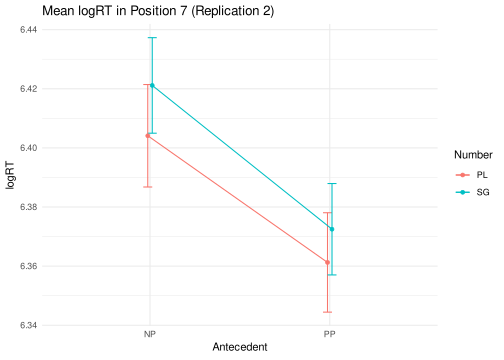
\includegraphics[height=4.5cm]{img/R2-results}\\
    \FigureCaption{Resultados da Replicação 2. As barras verticais representam os erros padrão das médias.}
  \end{columns}
\end{frame}

\begin{frame}{Estimativa do tamanho do efeito}
  \centering
  \includegraphics[height=5.5cm]{img/costa2013-effect-size-comparison}\\\
  \FigureCaption{Estimativas do tamanho do efeito de interação \textsc{np.sg} × \textsc{pp.sg} em Costa (2013) e em nossas replicações. As barras horizontais indicam o \textsc{ic} de 95\%. Figura adaptada de Costa (2022).}
\end{frame}

\begin{frame}{Interpretando nossos resultados}
  \begin{itemize}
  \item Não conseguimos replicar os resultados do Experimento 2 de Costa (2013) -- o que, de fato, está alinhado com sua hipótese original;
  \item Interpretamos isso como um caso de \alert{regressão à média}: o efeito inicial desapareceu em ambas as replicações, R1 e R2.
  \end{itemize}
\end{frame}

\begin{frame}{Conclusões da aula}
  \begin{itemize}
  \item \alert<1>{A psicolinguística é uma ciência}, porque segue o método científico.
  \item Esse método -- herdado em parte da psicologia --, entretanto, é fruto, \alert<2>{disputas, problemas e inovações}.
  \item Dentre outras causas, esses problemas derivam de \alert<3>{equívocos no uso e interpretação das ferramentas da estatística, bem como a falta de replicações}.
  \item Quando replicações são realizadas, \alert<4>{há sintomas de falsos positivos}, o que sugere a necessidade de inovações metodológicas (Sönning e Werner, 2021)
  \end{itemize}
\end{frame}

\section{Referências bibliográficas}

\begin{frame}[allowframebreaks]{Referências}
  \begin{thebibliography}{9}

  \bibitem{beraldo2024}
    BERALDO, Rafael Luis. \emph{Irreplicabilidade na linguística experimental: causas, consequências e intervenções metodológicas}. Tese de doutorado—Campinas: Universidade Estadual de Campinas, 2024.

  \bibitem{cohen1994}
    COHEN, Jacob. The earth is round (p < .05). \emph{American Psychologist}, v. 50, n. 12, 1994.

  \bibitem{costa2013}
    COSTA, Igor de Oliveira. \emph{Verbos meteorológicos no plural em orações relativas do português brasileiro: sintaxe e processamento}. Dissertação de mestrado—Rio de Janeiro: PUC-Rio, 2013.

  \bibitem{costa2022}
    COSTA, Igor de Oliveira. \emph{Poder estatístico e tamanho da amostra nos estudos em psicolinguística experimental: uma abordagem compreensiva usando simulações}. Rio de Janeiro, 15 set. 2022.

  \bibitem{costa2021}
    COSTA, Igor de Oliveira; AUGUSTO, Marina R. A. Um caso de concordância com tópico: a expressao de plural em verbos meteorológicos no interior de oracões relativas. In: \emph{VI Jornada de Estudos da Linguagem. Linguagem: teoria, análise e aplicacões}. Rio de Janeiro: Programa de Pós-graduação em Letras, 2011.

  \bibitem{fisher1955}
    FISHER, Ronald. Statistical Methods and Scientific Induction. \emph{Journal of the Royal Statistical Society Series B: Statistical Methodology}, v. 17, n. 1, p. 69–78, jan. 1955.

  \bibitem{fisher1935}
    FISHER, Ronald A. \emph{The design of experiments}. Edinburgh: Oliver and Boyd, 1935.

  \bibitem{ioannidis2005}
    IOANNIDIS, John P. A. Why most published research findings are false. \emph{PLoS Medicine}, v. 2, n. 8, p. e124, 30 ago. 2005.

  \bibitem{just1980}
    JUST, Marcel Adam; CARPENTER, Patricia A. A theory of reading: from eye fixations to comprehension. \emph{Psychological Review}, v. 87, n. 4, p. 28, 1980.

  \bibitem{kantowitz2009}
    KANTOWITZ, Barry H.; ROEDIGER III, Henry L.; ELMES, David G. \emph{Experimental Psychology}. 9. ed. Belmont: Wadsworth, 2009.

  \bibitem{nosek2020}
    NOSEK, Brian A.; ERRINGTON, Timothy M. What is replication? \emph{PLOS Biology}, v. 18, n. 3, p. e3000691, 27 mar. 2020.

  \bibitem{pashler2012}
    PASHLER, Harold; HARRIS, Christine R. Is the Replicability Crisis overblown? Three arguments examined. \emph{Perspectives on Psychological Science}, v. 7, n. 6, p. 531–536, 1 nov. 2012.

  \bibitem{popper2002}
    POPPER, Karl. \emph{The logic of scientific discovery}. London: Routledge, 2002.

  \bibitem{rosenthal1979}
    ROSENTHAL, Robert. The file drawer problem and tolerance for null results. \emph{Psychological Bulletin}, v. 86, n. 3, p. 638–641, maio 1979.

  \bibitem{sonning2021}
    SÖNNING, Lukas; WERNER, Valentin. The replication crisis, scientific revolutions, and linguistics. \emph{Linguistics}, v. 59, n. 5, p. 1179–1206, 27 set. 2021.

  \bibitem{vasishth2016}
    VASISHTH, Shravan; NICENBOIM, Bruno. Statistical methods for linguistic research: foundational ideas – Part I. \emph{Language and Linguistics Compass}, v. 10, n. 8, p. 349–369, ago. 2016.

  \end{thebibliography}
\end{frame}
\end{document}

% Local Variables:
% jinx-languages: "pt_BR"
% End:
